% !TeX spellcheck = en_US
\documentclass{beamer}
\usepackage[latin1]{inputenc}
\usepackage{dsfont}
\usepackage{color}
\usepackage{tabularx}
\usepackage{amssymb}

% % % % % FRAME STYLE

% NEW
%\usetheme{Frankfurt}
%\setbeamertemplate{navigation symbols}{}
%\setbeamertemplate{frametitle}[default][center]

% OLD
\setbeamertemplate{navigation symbols}{}
\setbeamertemplate{frametitle}{\vspace{5mm}\hspace{0mm}\insertframetitle}
%\setbeamertemplate{frametitle}[default][center]
\setbeamertemplate{footline}{\hfill\insertframenumber/\inserttotalframenumber\hspace{5mm}\vspace{5mm}}
\AtBeginSection[]
{
	\begin{frame}
		\frametitle{Agenda}
		\tableofcontents[currentsection]
	\end{frame}
}

\usefonttheme{structurebold}
\usecolortheme{dove}

% % % % % CUSTOM COMMANDS
\newcommand{\Empty}{\mbox{$\varnothing$}}
\newcommand{\NotEmpty}{\mbox{$\neg\varnothing$}}
\newcommand{\ToDo}{\textcolor{red}{TODO}}

% % % % % FRAMES

\begin{document}

	\title{Qualitative Spatial Reasoning over Line-Region Relations}
	\author{Leena and Sibel}
	\date{Knowledge Representation\\Seminar Presentation}
	
	\begin{frame}
		\titlepage
	\end{frame}
	
	\section{Motivation}
	
	\section{Background}
	
	\subsection{Lines and Regions}
	
	\subsection{Topological Parts of an Object}
	
	\subsection{9-Intersection}
	
	\section{Conceptual Neighborhood Models}
	
	\subsection{Snapshot Model}
	
%	\begin{frame}{Snapshot Model}
%		
%	\end{frame}
%	
%	\begin{frame}{Resulting Neighborhood Graph}
%		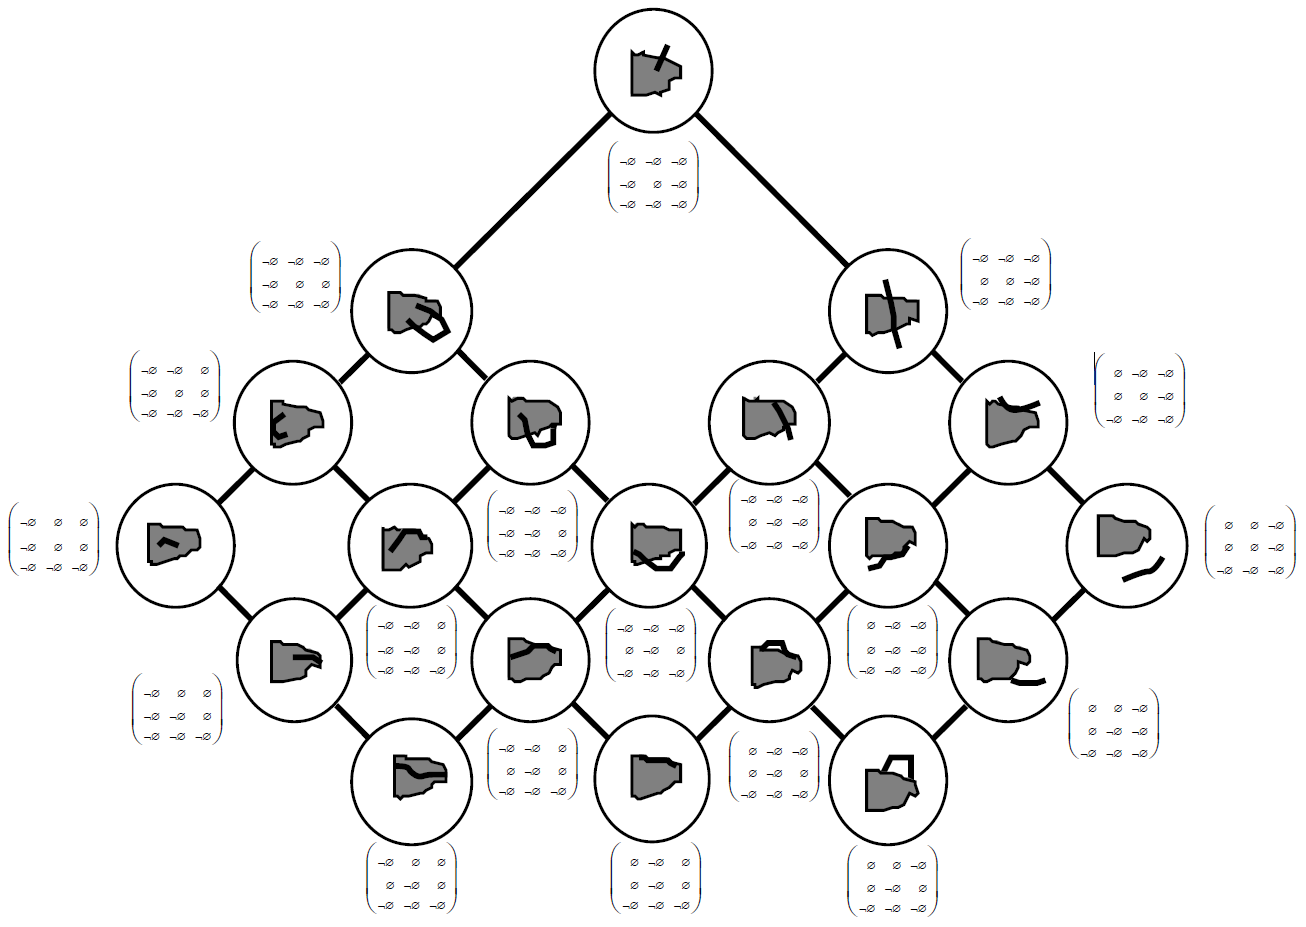
\includegraphics[width=\textwidth]{images/snapshot_model_neighborhood_graph.png}
%	\end{frame}
	
	\subsection{Smooth Transitions}
	
	\begin{frame}{Smooth Transitions}
		
		\begin{block}{Conceptual Neighborhood} A line-region relation is topologically different from another one by an infinitesimally small deformation of its geometry.
		\end{block}
		
		\begin{block}{Possible Changes} A total of four rules:
			\begin{itemize}
				\item Moving around a line's boundary nodes
				\begin{itemize}
					\item[Rule 1] Line's two boundary nodes intersect with same region part
					\item[Rule 2] Line's two boundary nodes intersect with different region part
				\end{itemize}
				\item Moving around a line's interior
				\begin{enumerate}
					\item[Rule 3] Extend line's interior-intersection partially
					\item[Rule 4] Reduce line's interior-intersection partially
				\end{enumerate}
			\end{itemize}
		\end{block}
		
		In terms of 9-Intersection, a smooth transition means that an intersection or its adjacent intersection gets changed from empty to non-empty, or reverse.
	\end{frame}
	
	\begin{frame}{Extent of a Line Part}
		Extent of a part $i$: Denoted by $ \#M[i, \_]$; number of non-empty intersections between $i$ and th three parts of the second object.
		Define extent of a part i Draw 9-intersection model on the board for reference
		
		\begin{itemize}
			\item The extent of a line's interior with respect to a region is in the interval of 1 to 3, the extent of the lines boundary is either 1 (if both nodes are located in the same region part) or 2 (if the nodes are located in different parts of the region), and the extent of a line's interior is always 3.
		\end{itemize}
	\end{frame}
	
	\begin{frame}{Moving the Line's Boundaries}
		\begin{block}{Rule 1}
			If the line's two boundaries intersect with the same region part, then extend the intersection to either of the adjacent region parts.
		\end{block}
		
		\begin{block}{Formalization}
			\centering $ \#M[\delta, \_] = 1 \Rightarrow
			\forall i (M[\delta, i] = \NotEmpty):
			M_{N}[\delta, \text{adjacent}(i)] := \NotEmpty $
		\end{block}
		
		\begin{block}{Example}
			%Moving one boundary of a line into an adjacent part of the region.
			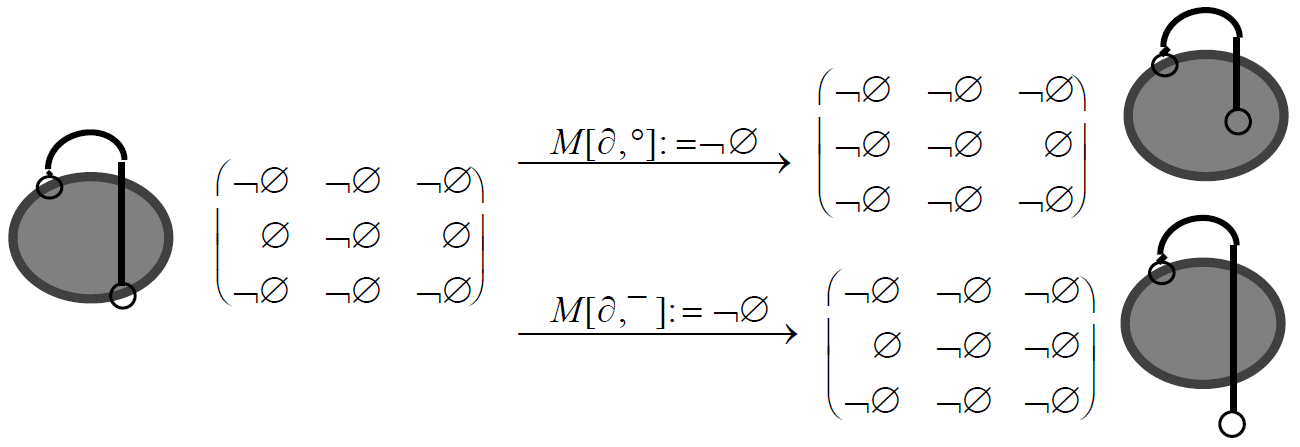
\includegraphics[width=\textwidth]{images/smooth_transitions_example_a.png}
		\end{block}
	\end{frame}
	
	\begin{frame}{Moving the Line's Boundaries}
		\begin{block}{Rule 2}
			If the line's two boundaries intersect with two different region parts then move either intersection to the adjacent region part.
		\end{block}
		
		\begin{block}{Formalization}
			\centering $ \#M[\delta,\_] = 2 \Rightarrow
			\forall i (M[\delta, i] = \NotEmpty):
			M_{N}[\delta, i] := \Empty \text{ \textbf{and} }
			M_{N}[\delta, \text{adjacent}(i)] := \NotEmpty $
		\end{block}
		
		\begin{block}{Example}
			%Moving either boundary into an adjacent region part.
			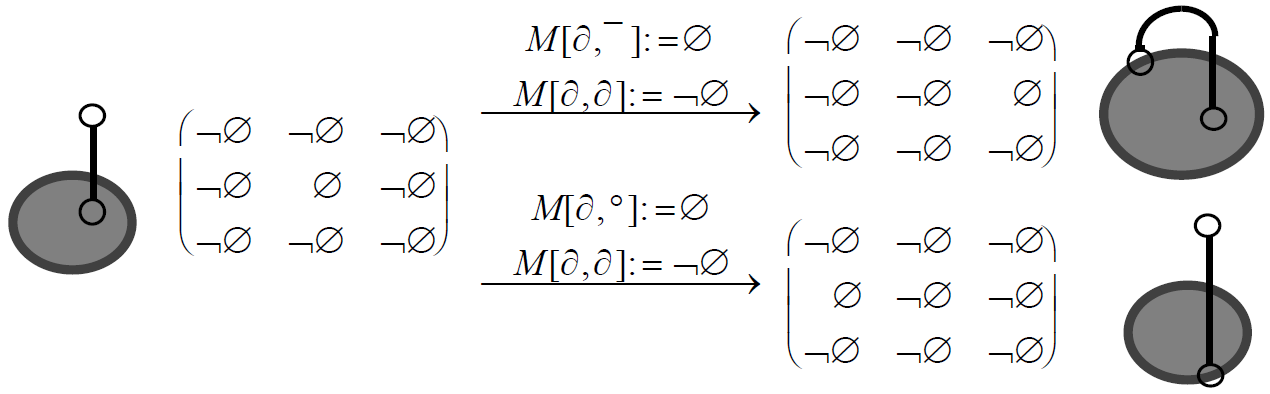
\includegraphics[width=\textwidth]{images/smooth_transitions_example_b.png}
		\end{block}
	\end{frame}
	
	\begin{frame}{Moving the Line's Interior}
		\begin{block}{Rule 1}
			Extend the line's interior-intersection to either of the adjacent region parts.
		\end{block}
		
		\begin{block}{Formalization}
			\centering $ \forall i (M[�, i] = \NotEmpty):
			M_{N}[�, \text{adjacent}(i)] := \NotEmpty $
		\end{block}
		
		\begin{block}{Example}
			%Moving the line's interior into an adjacent part of the region.
			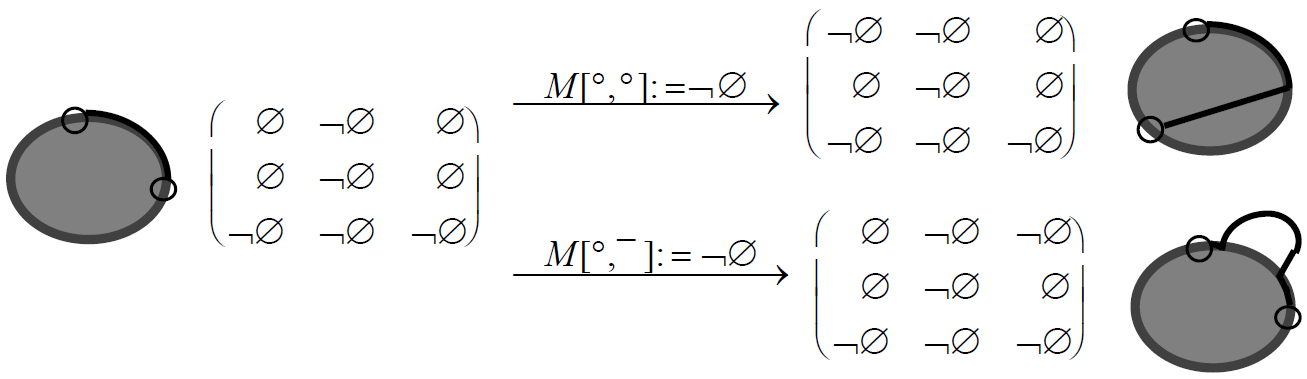
\includegraphics[width=\textwidth]{images/smooth_transitions_example_c.png}
		\end{block}
	\end{frame}
	
	\begin{frame}{Moving the Line's Interior}
		\begin{block}{Rule 2}
			Reduce the line's interior intersection on either of the adjacent region parts.
		\end{block}
		
		\begin{block}{Formalization}
			\centering
			$ \#M[�, \_] = 2 \Rightarrow
			\forall i (M[�, i] = \NotEmpty):
			M_{N}[�, i] := \Empty $
			$ \#M[�, \_] = 3 \Rightarrow
			\forall i (i \neq \delta):
			M_{N}[�, i] := \Empty $
		\end{block}
		
		\begin{block}{Example}
			%Moving the line's interior out of a part of the region.
			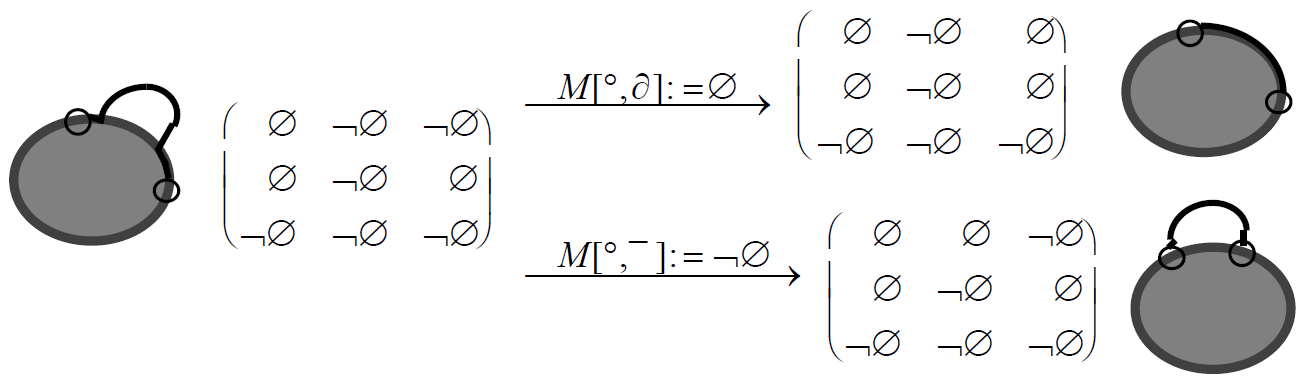
\includegraphics[width=\textwidth]{images/smooth_transitions_example_d.png}
		\end{block}
	\end{frame}
	
	\begin{frame}{Consistency Constraints}
		\begin{enumerate}
			\item If the line's interior intersects with the region's interior \textit{and} exterior, then the line's interior must also intersect with the region's boundary.
			\begin{center}
				$ M[�,�] = \NotEmpty \text{and} M[�,^{-}] = \NotEmpty \Rightarrow M[�,\delta] := \NotEmpty $
			\end{center}
			
			\item If the line's boundary intersects with the region's interior (exterior) then the line's interior must intersect with the region's interior (exterior) as well.
			\begin{center}
				$ M[\delta, �] = \NotEmpty M[�,�] := \NotEmpty $ \\
				$ M[\delta, ^{-}] = \NotEmpty M[�,^{-}] := \NotEmpty $
			\end{center}
		\end{enumerate}
		
	\end{frame}
	
	% NOTES:
	% The separate moves of the line's interior and boundaries are atomic operations that do not account for some of the properties of the objects and their embedding space and, therefore, may generate inconsistent 9-intersections for configurations that cannot be realized. In order to maintain connectivity among the line's boundaries and interior, it is necessary to assure the following \textbf{consistency constraint}: [1]. Likewise, in order to preserve the continuous-space property of $\mathcal{R}^{2}$, the following consistency constraint must be fulfilled: [2].
	
	\begin{frame}{Resulting Neighborhood Graph}
		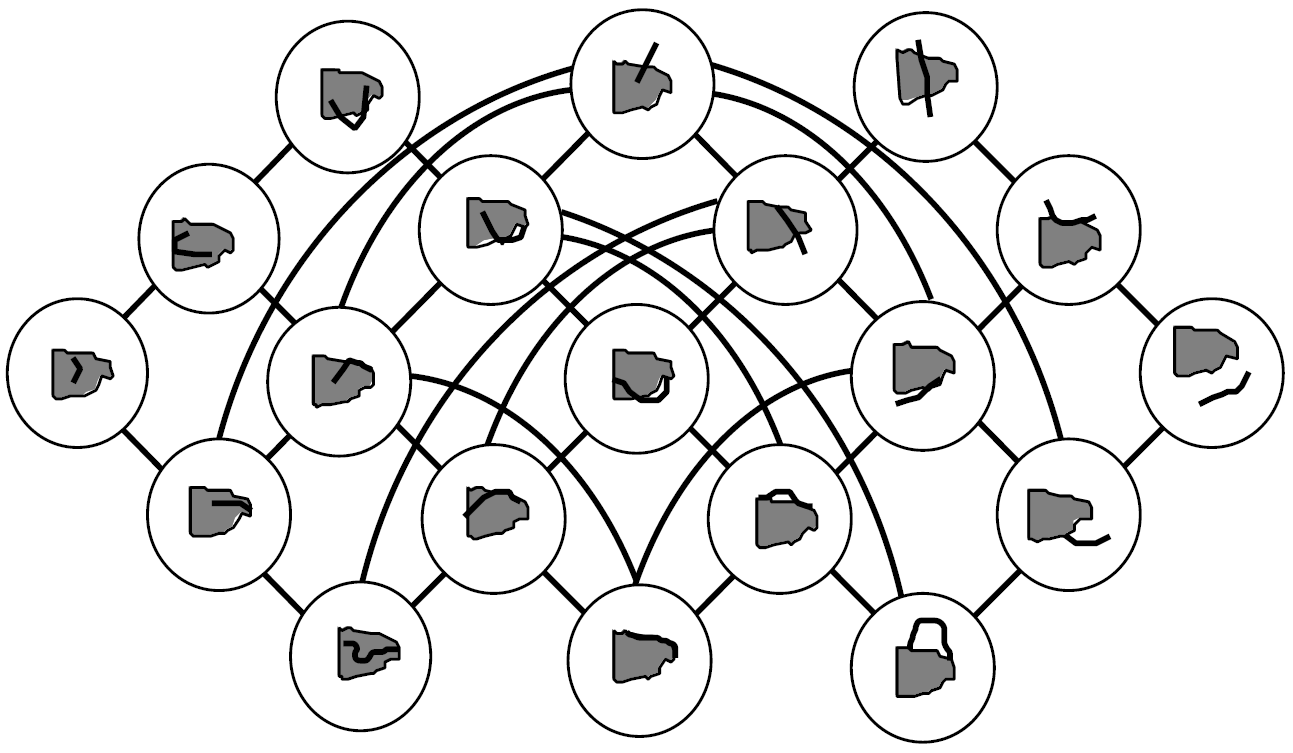
\includegraphics[width=\textwidth]{images/smooth_transitions_neighborhood_graph.png}
	\end{frame}
	
	% NOTES:
	% This graph resembles in most of its structure and properties the snapshot neighborhood graph. The difference between the two graphs are
	%\begin{itemize}
	%	\item the way in which conceptual neighbors are connected at the top,
	%	\item the additional links that run across the smooth transition graph.
	%\end{itemize}
	
	
	\section{Evaluation}
	
	\section{Conclusion}

	
	
	\begin{frame}{References}  
		\begin{thebibliography}{10}    
%			\beamertemplatebookbibitems
%			\bibitem{Diekert2013}
%			V.~Diekert, M.~Kufleitner, G.~Rosenberger.
%			\newblock {\em Diskrete Algebraische Methoden}. (Abschnitt 7.6)
%			\newblock Walter de Gruyter, 2013.
%			\beamertemplatearticlebibitems
%			\bibitem{Heller2008}
%			A.~Heller.
%			\newblock Ein Entscheidungsverfahren f�r die Presburger Arithmetik.
%			\newblock https://www4.in.tum.de/lehre/vorlesungen/perlen/SS08/\\Unterlagen/Presburger.pdf.
		\end{thebibliography}
	\end{frame}
\end{document}